\documentclass[12pt,a4paper]{article}

% Paquetes básicos
\usepackage[utf8]{inputenc}
\usepackage[T1]{fontenc}
\usepackage[english]{babel}
\usepackage{amsmath, amssymb}
%\usepackage{siunitx} 
\usepackage{graphicx}
\usepackage{float}
\usepackage{geometry}
\usepackage{xcolor}
\geometry{margin=2.5cm}
\usepackage{hyperref}
\usepackage{caption}
\usepackage{subcaption}
\usepackage{setspace}
\usepackage{multirow}
%\usepackage{minted}  
\usepackage{gensymb} 
\usepackage[backend=biber, style=ieee]{biblatex}
\usepackage[american, straightvoltages]{circuitikz}
\usepackage{csquotes}
\usepackage{indentfirst}
\addbibresource{references.bib}

\graphicspath{{Figures/}}
\onehalfspacing
\hypersetup{
    colorlinks  = true,
    linkcolor   = blue,    
    citecolor   = blue,
    urlcolor    = blue,
    filecolor   = blue
}

\begin{document}       
\renewcommand{\figureautorefname}{Fig.}
\renewcommand{\tableautorefname}{Tab.}
\renewcommand{\equationautorefname}{Eq.}


% Carátula personalizada
\begin{titlepage}
    \centering
    
\includegraphics[width=0.7\textwidth]{Fulgor Logo.png}\\[1.5cm]

    {\Large \textbf{FUNDACIÓN FULGOR} \\[0.5cm]}
    {\Large CMOS Course} \\[0.5cm]

    \rule{\textwidth}{0.5pt} \\[0.5cm]
    {\Large \textbf{Homework N°4} \\[0.3cm]}
    \rule{\textwidth}{0.5pt} \\[1cm]
    
\begin{tabular}{l l}
    \textbf{Professors:} & Camilo Estevez.\\
                         & Ramón Sarmiento.\\
    \\
    \textbf{Student:}    & Monja, Ernesto Joaquín (43.873.728)\\
\end{tabular} \\[5cm]

{\centering Year 2026 \par}

\end{titlepage}



% Índice
\tableofcontents
\newpage



\section{Introduction}                                          \label{sec_1}
This report analyzes and calculates the \textit{Differential Gain} of the circuit shown in \autoref{fig:fig_1}. 
\begin{figure}[H]
    \centering
    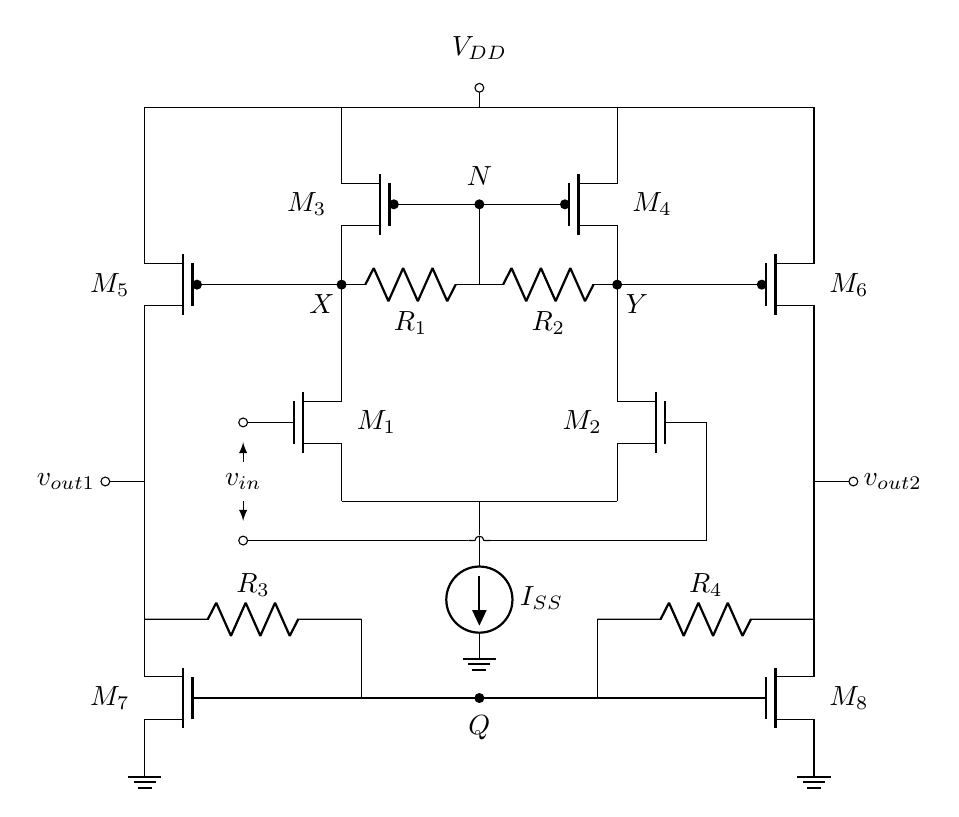
\begin{tikzpicture}[transform shape]
	% Paths, nodes and wires:
	\node[nmos](N1) at (-1.75, 0){} node[anchor=west] at (N1.text){$M_{1}$};
	\node[nmos, xscale=-1, yscale=-1](N2) at (1.75, 0){} node[anchor=east] at (N2.text){$M_{2}$};
	\draw (-1.75, -1) -- (-0.5, -1) -- (1.5, -1) -- (1.75, -1);
	\draw (0, -1.75) to[american current source, l={$I_{SS}$}] (0, -2.75);
	\draw (0, -2.75) -- (0, -3);
	\node[nmos](N3) at (4.25, -3.5){} node[anchor=west] at (N3.text){$M_{8}$};
	\node[pmos, xscale=-1, yscale=-1](N4) at (-1.75, 2.77){} node[anchor=east] at (N4.text){$M_{3}$};
	\node[pmos](N5) at (1.75, 2.77){} node[anchor=west] at (N5.text){$M_{4}$};
	\draw (-1.75, 2) -- (-1.75, 0.77);
	\draw (1.75, 2) -- (1.75, 0.77);
	\node[tlground] at (0, -3){};
	\draw (-1.75, -0.77) -| (-1.75, -1);
	\draw (-0.77, 2.77) -| (0.77, 2.77);
	\draw (0, 2.77) -- (0, 1.75);
	\draw (-0.25, 1.75) to[american resistor, l={$R_{1}$}] (-1.5, 1.75);
	\draw (1.5, 1.75) to[american resistor, l={$R_{2}$}] (0.25, 1.75);
	\draw (1.75, -0.77) -- (1.75, -1);
	\draw (-2.73, 0) -- (-3, 0);
	\node[pmos, xscale=-1, yscale=-1](N6) at (-4.25, 1.75){} node[anchor=east] at (N6.text){$M_{5}$};
	\draw (2.73, 0) -| (2.89, -0.25) -| (2.89, -1.5) -- (0.14, -1.5);
	\draw (-0.14, -1.5) -- (-3, -1.5);
	\node[jump crossing] at (0, -1.5){};
	\draw (0, -1.64) -| (0, -1.75);
	\draw (0, -1.36) -| (0, -1);
	\node[ocirc] at (-3, 0){};
	\node[ocirc] at (-3, -1.5){};
	\node[pmos](N7) at (4.25, 1.75){} node[anchor=west] at (N7.text){$M_{6}$};
	\node[nmos, xscale=-1, yscale=-1](N8) at (-4.25, -3.5){} node[anchor=east] at (N8.text){$M_{7}$};
	\draw (4.25, -2.73) -- (4.25, 1);
	\draw (-4.25, 1) -| (-4.25, -2.73);
	\draw (-3.27, -3.5) |- (3.27, -3.5);
	\node[tlground] at (-4.25, -4.5){};
	\node[tlground] at (4.25, -4.5){};
	\draw (-4.25, -4.27) -| (-4.25, -4.5);
	\draw (4.25, -4.27) -| (4.25, -4.5);
	\node[shape=rectangle, minimum width=0.715cm, minimum height=0.465cm](N9) at (-3, -0.75){} node[anchor=center] at (N9.text){$v_{in}$};
	\draw[-latex] (-3, -0.5) -- (-3, -0.25);
	\draw[-latex] (-3, -1) -- (-3, -1.25);
	\draw (-1.75, 1.75) -- (-1.5, 1.75);
	\draw (-0.25, 1.75) -- (0.25, 1.75);
	\draw (1.5, 1.75) -- (1.75, 1.75);
	\draw (3.27, 1.75) |- (1.75, 1.75);
	\draw (-3.27, 1.75) -- (-1.75, 1.75);
	\draw (-1.75, 4) -- (1.75, 4) -| (1.75, 3.54);
	\draw (-4.25, -2.5) to[american resistor, l={$R_{3}$}] (-1.5, -2.5);
	\draw (-1.5, -2.5) -- (-1.5, -2.5) -| (-1.5, -3.5);
	\draw (1.5, -2.5) to[american resistor, l={$R_{4}$}] (4.25, -2.5);
	\draw (1.5, -2.5) -- (1.5, -2.5) -- (1.5, -3.5);
	\draw (-4.25, -0.75) -- (-4.75, -0.75);
	\draw (4.25, -0.75) -- (4.75, -0.75);
	\node[ocirc] at (-4.75, -0.75){};
	\node[ocirc] at (4.75, -0.75){};
	\node[shape=rectangle, minimum width=0.715cm, minimum height=0.465cm](N10) at (-5.25, -0.75){} node[anchor=center] at (N10.text){$v_{out1}$};
	\node[shape=rectangle, minimum width=0.715cm, minimum height=0.465cm](N11) at (5.25, -0.75){} node[anchor=center] at (N11.text){$v_{out2}$};
	\draw (-1.75, 4) -- (-1.75, 3.54);
	\draw (4.25, 2.52) -| (4.25, 4) -- (1.75, 4);
	\draw (-4.25, 2.52) -| (-4.25, 4) -- (-1.75, 4);
	\draw (0, 4) -| (0, 4.25);
	\node[ocirc] at (0, 4.25){};
	\node[shape=rectangle, minimum width=0.715cm, minimum height=0.465cm](N12) at (0, 4.75){} node[anchor=center] at (N12.text){$V_{DD}$};
	\node[circ] at (-1.75, 1.75){};
	\node[circ] at (1.75, 1.75){};
	\node[shape=rectangle, minimum width=0.715cm, minimum height=0.465cm](N13) at (-2, 1.5){} node[anchor=center] at (N13.text){$X$};
	\node[shape=rectangle, minimum width=0.715cm, minimum height=0.465cm](N14) at (2, 1.5){} node[anchor=center] at (N14.text){$Y$};
	\node[circ] at (0, 2.77){};
	\node[shape=rectangle, minimum width=0.777cm, minimum height=0.695cm](N15) at (0, 3.135){} node[anchor=center] at (N15.text){$N$};
	\node[circ] at (0, -3.5){};
	\node[shape=rectangle, minimum width=0.777cm, minimum height=0.715cm](N16) at (0, -3.875){} node[anchor=center] at (N16.text){$Q$};
\end{tikzpicture}
    \caption{Circuit proposed to analyze.} 
    \label{fig:fig_1}
\end{figure}

The report will present details of the step-by-step calculation of the differential voltage gain under the assumptions that: Channel-length modulation is negligible ($\lambda = 0$) for all transistors and thus $r_{0} = \infty \, [\Omega]$ ; $R_{1}$ is equal to $R_{2}$, and $R_{3}$ is equal to $R_{4}$ and all transistors have the same $W/L$ relationship.



\section{Circuit Analysis}                                      \label{sec_2}
The circuit shown in \autoref{fig:fig_1} consist of a two-stage fully differential \textit{CMOS} amplifier:
\begin{itemize}
    \item The first stage comprises a differential pair ($M_{1}$ and $M_{2}$) biased by a tail current source $I_{SS}$. The load for this initial stage consists of a symmetric network formed by resistors $R_{1}$ and $R_{2}$ alongside active \textit{PMOS} devices $M_{3}$ and $M_{4}$.
    \item The second stage is composed of common-source amplifiers ($M_{5}$ and $M_{6}$) loaded by an output network consisting of resistors $R_{3}$ and $R_{4}$, and \textit{NMOS} current sources $M_{7}$ and $M_{8}$.
\end{itemize}

The following subsections will analyze these two stages separately based on the half circuit model proposed by Bezhad Razavi. \cite{b1} Note that since the circuit is perfectly symmetric and we are evaluating purely differential signals, the nodes connecting symmetric components become \textit{AC} virtual grounds.



\subsection{First Stage Gain}                                   \label{sec_2.1}
This first stage is a differential pair composed of $M_{1}$ and $M_{2}$ biased with the tail current source $I_{SS}$ as mentioned in \autoref{sec_2}. Note that the input signal is applied differentially, meaning:
\begin{equation}
    \begin{cases}
        v_{in1} =  \frac{v_{in}}{2} \\
        v_{in2} = -\frac{v_{in}}{2}
    \end{cases}
    \label{eq_1}
\end{equation}

The midpoint between $R_{1}$ and $R_{2}$ (labeled as node \textit{N} in \autoref{fig:fig_1}) is an \textit{AC} virtual ground. Consequently, the gates of $M_{3}$ and $M_{4}$ are tied to zero \textit{AC} voltage. Since the sources of $M_{3}$ and $M_{4}$ are connected to $V_{DD}$, which is also an \textit{AC} ground, we have that:
\begin{equation}
    v_{GS3} = v_{GS4} = 0 \, [V]
    \label{eq_2}
\end{equation}
 
With $\lambda = 0$, the output resistance of these transistors is infinite ($r_{o3} = r_{o4} = \infty \, [\Omega]$). Therefore, the equivalent impedance looking into the load at node \textit{X} is simply the resistor $R_{1}$ connected to the AC virtual ground such that the small-signal voltage at this node is given by:
\begin{equation}
    v_{X} = -g_{m1} \cdot R_{1} \cdot \frac{v_{in}}{2}
    \label{eq_3}
\end{equation}

This result can be verified with the \textit{Example 4.12} of Bezhad Razavi's book: \textit{Design of Analog CMOS Integrated Circuits}, as shown in \autoref{fig:fig_2}.
\begin{figure}[H]
    \centering
    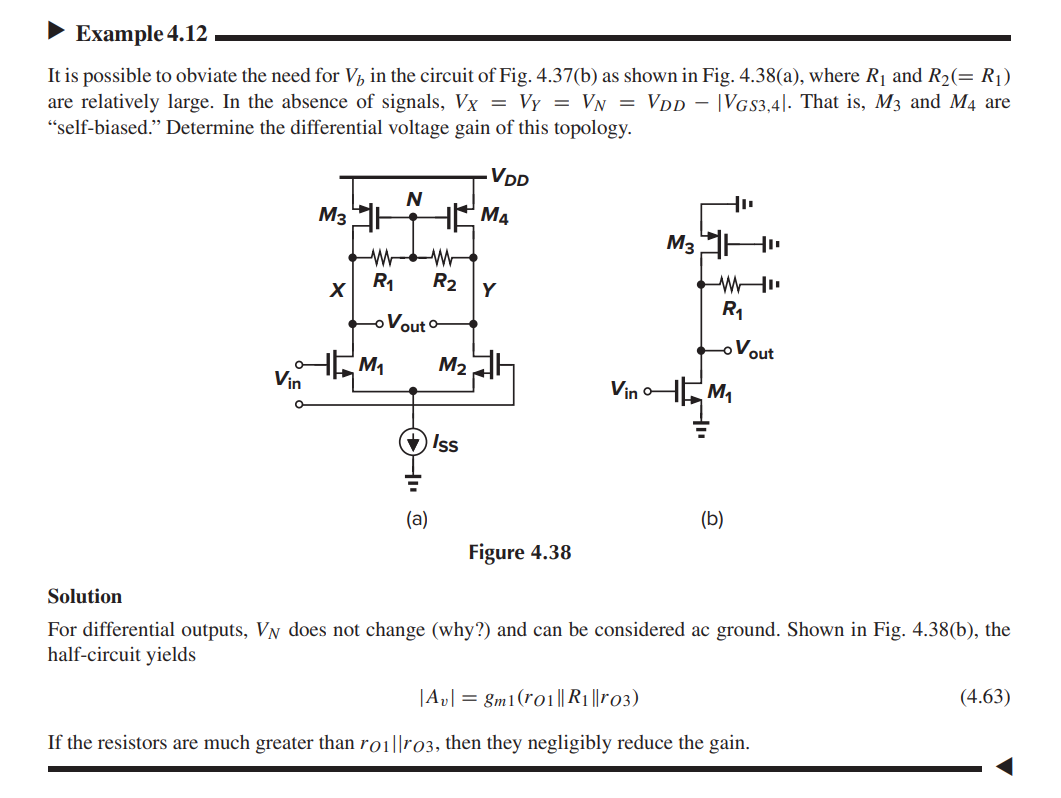
\includegraphics[width=0.738\linewidth]{Figure 2.png}
    \caption{Stage 1 Gain verification. \cite[p. 124]{b2}}
    \label{fig:fig_2}
\end{figure}



\subsection{Second Stage Gain}                              \label{sec_2.2}
The second stage consists of $M_{5}$ operating as a \textit{Common-Source PMOS} amplifier driven by its input voltage $v_{X}$. The load network at the output node $V_{out1}$ consists of $R_{3}$ and $M_{7}$.

Similar to the first stage, the midpoint between $R_{3}$ and $R_{4}$ (node \textit{Q}) acts as an \textit{AC} virtual ground for differential signals. This places the gate of $M_{7}$ at \textit{AC} ground, resulting in $v_{GS7} = 0$. 

Once again, given that $\lambda = 0$, $M_{7}$ acts as an ideal open circuit for small signals ($r_{o7} = \infty \, [\Omega]$) and thus, the equivalent load for $M_{5}$ is therefore just the resistor $R_{3}$. Therefore, the output voltage at $v_{out1}$ is given by \autoref{eq_4}.
\begin{equation}
    v_{out1} = -g_{m5} \cdot R_{3} \cdot v_{X}
    \label{eq_4}
\end{equation}

Replacing $v_{X}$ in \autoref{eq_4} with the result obtained in \autoref{eq_3} we have:
\begin{equation}
    v_{out1} = -g_{m5} \cdot R_{3} \cdot \left(-g_{m1} \cdot R_{1} \cdot \frac{v_{in}}{2} \right)
    \label{eq_5}
\end{equation}
\begin{equation}
    v_{out1} = g_{m1} \cdot g_{m5} \cdot R_{1} \cdot R_{3} \cdot \frac{v_{in}}{2}
    \label{eq_6}
\end{equation}

By symmetry, the voltage at the complementary output $V_{out2}$ is:
\begin{equation}
    v_{out2} = -g_{m2} \cdot g_{m6} \cdot R_{2} \cdot R_{4} \cdot \frac{v_{in}}{2}
    \label{eq_7}
\end{equation}

where given the assumptions made in \autoref{sec_1}, another way of writing \autoref{eq_7} is:
\begin{equation}
    v_{out2} = -g_{m1} \cdot g_{m5} \cdot R_{1} \cdot R_{3} \cdot \frac{v_{in}}{2}
    \label{eq_8}
\end{equation}



\subsection{Total Differential Gain}
The total differential output voltage is given by:
\begin{equation}
    v_{out,diff} = v_{out1} - v_{out2}
    \label{eq_9}
\end{equation}

where substituting \autoref{eq_6} and \autoref{eq_8} into \autoref{eq_9}, we have:
\begin{equation}
    v_{out,diff} = g_{m1} \cdot g_{m5} \cdot R_{1} \cdot R_{3} \cdot v_{in}
    \label{eq_10}
\end{equation}

Finally, we have that the differential voltage gain is:
\begin{equation}
    A_v = \frac{v_{out,diff}}{v_{in}} = g_{m1} \cdot g_{m5} \cdot R_{1} \cdot R_{3}
    \label{eq_11}
\end{equation}



\section{Conclusion}                                            \label{sec_3}
The derived differential voltage gain obtained in \autoref{eq_11}, demonstrates a highly coherent physical behavior for this two-stage topology. Under purely differential excitation, the nodes driving the Common-Mode Feedback (\textit{CMFB}) transistors ($M_{3}$, $M_{4}$, $M_{7}$, and $M_{8}$) act as \textit{AC} virtual grounds, effectively disabling these active devices in the small-signal regime. Coupled with the $\lambda = 0$ constraint, which yields infinite intrinsic output resistances, all parasitic loading effects vanish entirely. This logically reduces each amplification stage to an ideal transconductor driving solely its respective \textit{CMFB} sensing resistor. Thus, the overall performance perfectly reflects a cascade of two unattenuated common-source amplifiers.



\printbibliography[heading=bibintoc, title={4 \, Bibliography}]
\end{document}